% Options for packages loaded elsewhere
\PassOptionsToPackage{unicode}{hyperref}
\PassOptionsToPackage{hyphens}{url}
%
\documentclass[
]{article}
\usepackage{lmodern}
\usepackage{amsmath}
\usepackage{ifxetex,ifluatex}
\ifnum 0\ifxetex 1\fi\ifluatex 1\fi=0 % if pdftex
  \usepackage[T1]{fontenc}
  \usepackage[utf8]{inputenc}
  \usepackage{textcomp} % provide euro and other symbols
  \usepackage{amssymb}
\else % if luatex or xetex
  \usepackage{unicode-math}
  \defaultfontfeatures{Scale=MatchLowercase}
  \defaultfontfeatures[\rmfamily]{Ligatures=TeX,Scale=1}
\fi
% Use upquote if available, for straight quotes in verbatim environments
\IfFileExists{upquote.sty}{\usepackage{upquote}}{}
\IfFileExists{microtype.sty}{% use microtype if available
  \usepackage[]{microtype}
  \UseMicrotypeSet[protrusion]{basicmath} % disable protrusion for tt fonts
}{}
\makeatletter
\@ifundefined{KOMAClassName}{% if non-KOMA class
  \IfFileExists{parskip.sty}{%
    \usepackage{parskip}
  }{% else
    \setlength{\parindent}{0pt}
    \setlength{\parskip}{6pt plus 2pt minus 1pt}}
}{% if KOMA class
  \KOMAoptions{parskip=half}}
\makeatother
\usepackage{xcolor}
\IfFileExists{xurl.sty}{\usepackage{xurl}}{} % add URL line breaks if available
\IfFileExists{bookmark.sty}{\usepackage{bookmark}}{\usepackage{hyperref}}
\hypersetup{
  pdftitle={Gestion de Portefeuille},
  pdfauthor={Patrick Hénaff},
  hidelinks,
  pdfcreator={LaTeX via pandoc}}
\urlstyle{same} % disable monospaced font for URLs
\usepackage[margin=1in]{geometry}
\usepackage{color}
\usepackage{fancyvrb}
\newcommand{\VerbBar}{|}
\newcommand{\VERB}{\Verb[commandchars=\\\{\}]}
\DefineVerbatimEnvironment{Highlighting}{Verbatim}{commandchars=\\\{\}}
% Add ',fontsize=\small' for more characters per line
\usepackage{framed}
\definecolor{shadecolor}{RGB}{248,248,248}
\newenvironment{Shaded}{\begin{snugshade}}{\end{snugshade}}
\newcommand{\AlertTok}[1]{\textcolor[rgb]{0.94,0.16,0.16}{#1}}
\newcommand{\AnnotationTok}[1]{\textcolor[rgb]{0.56,0.35,0.01}{\textbf{\textit{#1}}}}
\newcommand{\AttributeTok}[1]{\textcolor[rgb]{0.77,0.63,0.00}{#1}}
\newcommand{\BaseNTok}[1]{\textcolor[rgb]{0.00,0.00,0.81}{#1}}
\newcommand{\BuiltInTok}[1]{#1}
\newcommand{\CharTok}[1]{\textcolor[rgb]{0.31,0.60,0.02}{#1}}
\newcommand{\CommentTok}[1]{\textcolor[rgb]{0.56,0.35,0.01}{\textit{#1}}}
\newcommand{\CommentVarTok}[1]{\textcolor[rgb]{0.56,0.35,0.01}{\textbf{\textit{#1}}}}
\newcommand{\ConstantTok}[1]{\textcolor[rgb]{0.00,0.00,0.00}{#1}}
\newcommand{\ControlFlowTok}[1]{\textcolor[rgb]{0.13,0.29,0.53}{\textbf{#1}}}
\newcommand{\DataTypeTok}[1]{\textcolor[rgb]{0.13,0.29,0.53}{#1}}
\newcommand{\DecValTok}[1]{\textcolor[rgb]{0.00,0.00,0.81}{#1}}
\newcommand{\DocumentationTok}[1]{\textcolor[rgb]{0.56,0.35,0.01}{\textbf{\textit{#1}}}}
\newcommand{\ErrorTok}[1]{\textcolor[rgb]{0.64,0.00,0.00}{\textbf{#1}}}
\newcommand{\ExtensionTok}[1]{#1}
\newcommand{\FloatTok}[1]{\textcolor[rgb]{0.00,0.00,0.81}{#1}}
\newcommand{\FunctionTok}[1]{\textcolor[rgb]{0.00,0.00,0.00}{#1}}
\newcommand{\ImportTok}[1]{#1}
\newcommand{\InformationTok}[1]{\textcolor[rgb]{0.56,0.35,0.01}{\textbf{\textit{#1}}}}
\newcommand{\KeywordTok}[1]{\textcolor[rgb]{0.13,0.29,0.53}{\textbf{#1}}}
\newcommand{\NormalTok}[1]{#1}
\newcommand{\OperatorTok}[1]{\textcolor[rgb]{0.81,0.36,0.00}{\textbf{#1}}}
\newcommand{\OtherTok}[1]{\textcolor[rgb]{0.56,0.35,0.01}{#1}}
\newcommand{\PreprocessorTok}[1]{\textcolor[rgb]{0.56,0.35,0.01}{\textit{#1}}}
\newcommand{\RegionMarkerTok}[1]{#1}
\newcommand{\SpecialCharTok}[1]{\textcolor[rgb]{0.00,0.00,0.00}{#1}}
\newcommand{\SpecialStringTok}[1]{\textcolor[rgb]{0.31,0.60,0.02}{#1}}
\newcommand{\StringTok}[1]{\textcolor[rgb]{0.31,0.60,0.02}{#1}}
\newcommand{\VariableTok}[1]{\textcolor[rgb]{0.00,0.00,0.00}{#1}}
\newcommand{\VerbatimStringTok}[1]{\textcolor[rgb]{0.31,0.60,0.02}{#1}}
\newcommand{\WarningTok}[1]{\textcolor[rgb]{0.56,0.35,0.01}{\textbf{\textit{#1}}}}
\usepackage{graphicx}
\makeatletter
\def\maxwidth{\ifdim\Gin@nat@width>\linewidth\linewidth\else\Gin@nat@width\fi}
\def\maxheight{\ifdim\Gin@nat@height>\textheight\textheight\else\Gin@nat@height\fi}
\makeatother
% Scale images if necessary, so that they will not overflow the page
% margins by default, and it is still possible to overwrite the defaults
% using explicit options in \includegraphics[width, height, ...]{}
\setkeys{Gin}{width=\maxwidth,height=\maxheight,keepaspectratio}
% Set default figure placement to htbp
\makeatletter
\def\fps@figure{htbp}
\makeatother
\setlength{\emergencystretch}{3em} % prevent overfull lines
\providecommand{\tightlist}{%
  \setlength{\itemsep}{0pt}\setlength{\parskip}{0pt}}
\setcounter{secnumdepth}{-\maxdimen} % remove section numbering
\usepackage[utf8]{inputenc}
\usepackage{float}
\floatplacement{figure}{H}
\usepackage{float}
\usepackage{booktabs}
\usepackage{longtable}
\usepackage{array}
\usepackage{multirow}
\usepackage{wrapfig}
\usepackage{colortbl}
\usepackage{pdflscape}
\usepackage{tabu}
\usepackage{threeparttable}
\usepackage{threeparttablex}
\usepackage[normalem]{ulem}
\usepackage{makecell}
\usepackage{xcolor}
\ifluatex
  \usepackage{selnolig}  % disable illegal ligatures
\fi

\title{Gestion de Portefeuille}
\usepackage{etoolbox}
\makeatletter
\providecommand{\subtitle}[1]{% add subtitle to \maketitle
  \apptocmd{\@title}{\par {\large #1 \par}}{}{}
}
\makeatother
\subtitle{TP-4: Impact de la matrice de covariance dans le modèle MV}
\author{Patrick Hénaff}
\date{Février-Mars 2021}

\begin{document}
\maketitle

\hypertarget{donnuxe9es}{%
\section{Données}\label{donnuxe9es}}

On utilise la base de données ``MultiAsset'' du paquet FRAPO:

\begin{Shaded}
\begin{Highlighting}[]
\FunctionTok{library}\NormalTok{(FRAPO)}
\FunctionTok{data}\NormalTok{(MultiAsset)}
\NormalTok{R }\OtherTok{\textless{}{-}} \FunctionTok{returnseries}\NormalTok{(MultiAsset, }\AttributeTok{percentage=}\NormalTok{F, }\AttributeTok{trim=}\NormalTok{T)}
\end{Highlighting}
\end{Shaded}

Quelques statistiques descriptives sont résumées ci-dessous:

\begin{table}[H]

\caption{\label{tab:show-stats}Summary Statistics}
\centering
\begin{tabular}[t]{lrrrr}
\toprule
  & mean & std dev & skewness & kurtosis\\
\midrule
GSPC & 0.0007196 & 0.0483492 & -0.8809988 & 1.7602430\\
RUA & 0.0011323 & 0.0503202 & -0.8975063 & 1.8397675\\
GDAXI & 0.0046327 & 0.0597951 & -0.9841812 & 1.9749395\\
FTSE & 0.0018748 & 0.0437702 & -0.6912771 & 0.4962667\\
N225 & -0.0030518 & 0.0623081 & -1.0447685 & 2.8567460\\
\addlinespace
EEM & 0.0085561 & 0.0807882 & -0.7309404 & 1.2765558\\
DJCBTI & 0.0037850 & 0.0167642 & 0.7542986 & 2.7505223\\
GREXP & 0.0037178 & 0.0101831 & 0.1244254 & -0.4231236\\
BG05.L & 0.0013854 & 0.0151824 & 0.2047405 & 1.1789559\\
GLD & 0.0158004 & 0.0547407 & -0.4762910 & 0.7606515\\
\bottomrule
\end{tabular}
\end{table}

~

\hypertarget{etude-de-la-matrice-de-covariance}{%
\subsection{Etude de la matrice de
covariance}\label{etude-de-la-matrice-de-covariance}}

On se propose d'étudier la matrice de covariance à l'aide de la formule
de Stevens pour la matrice d'information \(\mathcal{I} = \Sigma^{-1}\).

\begin{itemize}
\tightlist
\item
  Pour chaque actif, estimer le modèle
\end{itemize}

\[
R_{i,t} = \beta_0 + \beta_i^T R_t^{(-i)} + \epsilon_{i,t}
\] avec \(R_t^{(-i)}\) vecteur de rendement de tous les actifs sauf
l'actif \(i\), \(\epsilon_{i,t} \sim \mathcal{N}(0, s_i^2)\)

\begin{verbatim}
##                    GSPC           RUA        GDAXI          FTSE         N225
## Intercept -0.0003723292  0.0003145585  0.007554474 -5.117019e-06 -0.006116991
## GSPC       0.0000000000  0.9944359962 -0.489100528  6.433106e-01 -2.277604558
## RUA        0.9786625921  0.0000000000  0.902956260 -3.099280e-01  2.376140673
## GDAXI     -0.0071170223  0.0133509066  0.000000000  2.084721e-01  0.290168646
## FTSE       0.0188581255 -0.0092317173  0.419977032  0.000000e+00  0.325262898
## N225      -0.0144138055  0.0152797528  0.126197462  7.021939e-02  0.000000000
## EEM       -0.0080378664  0.0141739831  0.080295840  1.474742e-01  0.110950338
## DJCBTI     0.0616101124 -0.0527297391 -0.242018201 -5.937445e-02 -0.156916259
## GREXP     -0.0353573242  0.0304397687 -0.647076213  1.739383e-01 -0.143153045
## BG05.L    -0.0053052277 -0.0038080739  0.512956121  1.156949e-01  0.114462375
## GLD       -0.0055844066  0.0047264909 -0.131036034 -5.237503e-02  0.004920328
##                    EEM        DJCBTI        GREXP       BG05.L          GLD
## Intercept  0.001031376  0.0006139235  0.002767243 -0.002184974  0.008845179
## GSPC      -0.927867482  0.6719678083 -0.181516577 -0.062625394 -1.112069220
## RUA        1.610249722 -0.5659893271  0.153792233 -0.044239271  0.926295957
## GDAXI      0.134877160 -0.0384100340 -0.048338429  0.088110337 -0.379704480
## FTSE       0.499044061 -0.0189833929  0.026176406  0.040034875 -0.305743214
## N225       0.081053940 -0.0108309050 -0.004650909  0.008550855  0.006200821
## EEM        0.000000000 -0.0290964290 -0.001658718  0.007940600  0.682663686
## DJCBTI    -0.307955804  0.0000000000  0.253450624  0.542474249  1.226678966
## GREXP     -0.037297589  0.5384593558  0.000000000  0.377600655 -0.257582799
## BG05.L     0.077651889  0.5012208699  0.164218921  0.000000000 -0.338107962
## GLD        0.395728368  0.0671850430 -0.006640472 -0.020042277 -0.338107962
\end{verbatim}

\begin{itemize}
\tightlist
\item
  Trier les modèles par \(R_i^2\) décroissant. En déduire les actifs qui
  sont susceptibles de recevoir un poids important dans le portefeuille
  optimal MV.
\end{itemize}

\begin{table}[H]

\caption{\label{tab:unnamed-chunk-3}Asset sorted by variance of their modelisation in decreasing order}
\centering
\begin{tabular}[t]{lrr}
\toprule
  & Résidual variance & Variance\\
\midrule
GLD & 0.0018018 & 0.0597104\\
N225 & 0.0014297 & 0.0059093\\
EEM & 0.0010445 & 0.0023558\\
GDAXI & 0.0006218 & 0.0103910\\
FTSE & 0.0003087 & 0.0018289\\
\addlinespace
BG05.L & 0.0001068 & 0.0001406\\
DJCBTI & 0.0000987 & 0.0001465\\
GREXP & 0.0000465 & 0.0004547\\
RUA & 0.0000092 & 0.0024898\\
GSPC & 0.0000090 & 0.0024083\\
\bottomrule
\end{tabular}
\end{table}

Les poids des actifs étant inversement proportionnels à la variance de
leur modélisation (mieux un actif est modélisé plus on lui donne un fort
poids dans notre portefeuille). Ainsi, le modèle MV donnera des poids de
plus en plus fort à mesure que l'on descend dans le tableau.

\begin{itemize}
\tightlist
\item
  Calculer les poids optimaux du modèle MV, et comparer avec les
  résultats des régressions.
\end{itemize}

On considère que le risk free rate vaut 3\%.

\begin{verbatim}
## Warning in plot.xy(xy.coords(x, y), type = type, ...): "lwbd" is not a graphical
## parameter
\end{verbatim}

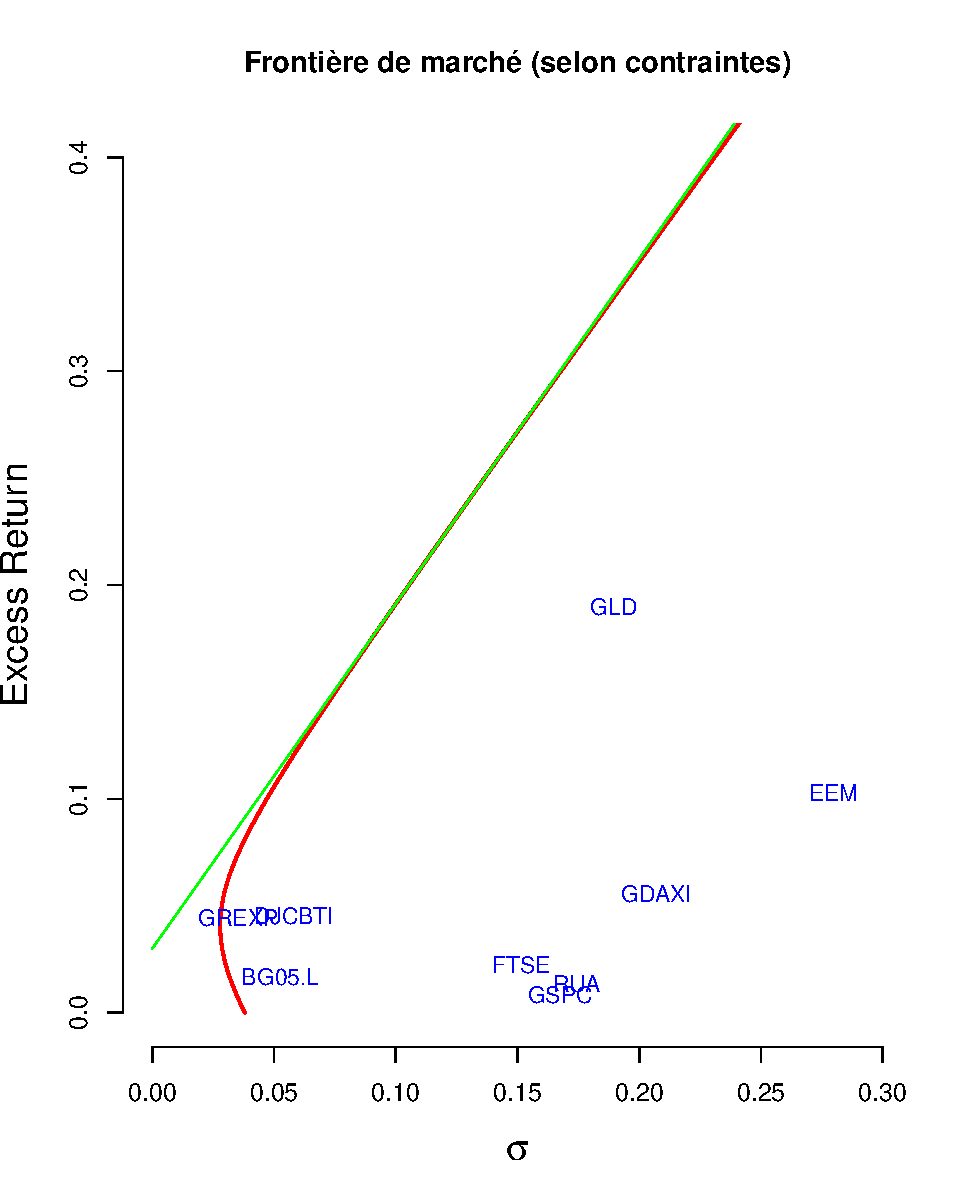
\includegraphics{TP-4-E_files/figure-latex/unnamed-chunk-4-1}

\begin{table}

\caption{\label{tab:unnamed-chunk-5}Composition du portefeuille optimal selon modèle MV}
\centering
\begin{tabular}[t]{lr}
\toprule
  & Proportion (\%)\\
\midrule
GSPC & -336.05\\
RUA & 264.52\\
GDAXI & 75.46\\
FTSE & -3.84\\
N225 & -35.99\\
\addlinespace
EEM & 16.48\\
DJCBTI & 67.16\\
GREXP & 182.74\\
BG05.L & -160.93\\
GLD & 30.44\\
\bottomrule
\end{tabular}
\end{table}

\hypertarget{interpretation}{%
\subsubsection{Interpretation}\label{interpretation}}

Pour les trois plus gros poids en valeurs absolues, on retrouve bien les
actifs aillant les variances résiduelles les plus faible. En revanche,
l'ordre est chamboulé pour le reste des actifs car les poids ne sont pas
calculé qu'à partir de cette variance résiduelle. Ainsi, d'autres
facteurs deviennent prépondérants.

\hypertarget{lien-avec-lacp}{%
\subsection{Lien avec l'ACP}\label{lien-avec-lacp}}

\begin{itemize}
\tightlist
\item
  Effectuer une ACP de la matrice de covariance des rendements.
\end{itemize}

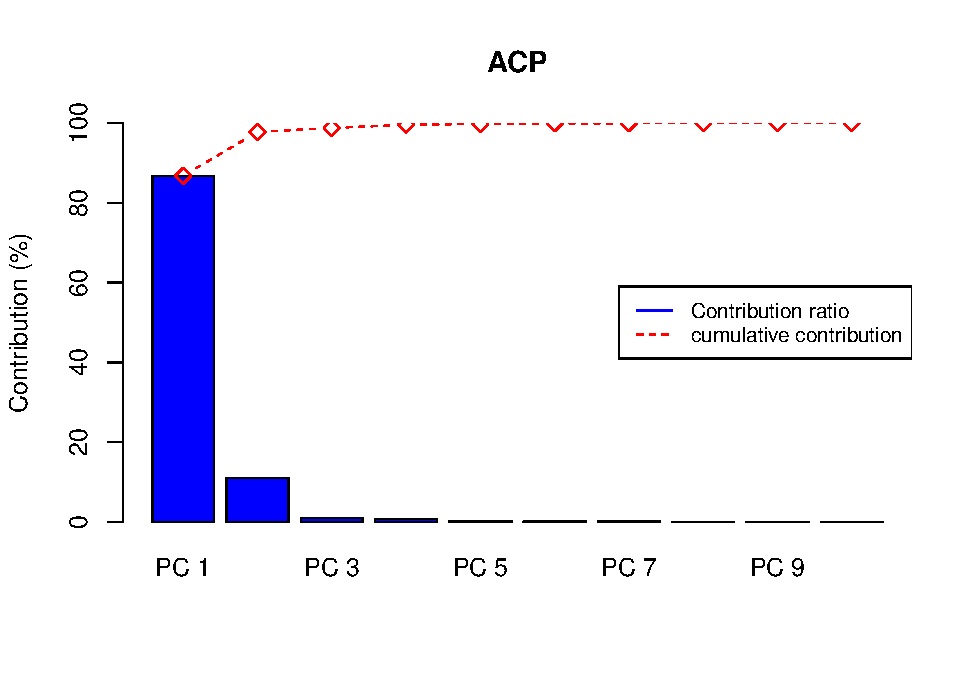
\includegraphics{TP-4-E_files/figure-latex/unnamed-chunk-6-1}

\begin{table}[H]

\caption{\label{tab:unnamed-chunk-7}Composition of PCs}
\centering
\begin{tabular}[t]{lrrrrrrrrrr}
\toprule
Tickers & PC1 & PC2 & PC3 & PC4 & PC5 & PC6 & PC7 & PC8 & PC9 & PC10\\
\midrule
GSPC & -33.74 & -4.03 & -10.63 & 29.08 & -19.91 & 23.75 & 38.92 & -4.99 & -40.13 & 61.45\\
RUA & -33.76 & -4.32 & -10.62 & 26.42 & -19.25 & 21.79 & 37.75 & -2.64 & 71.53 & -25.23\\
GDAXI & -33.64 & 7.12 & -22.21 & 3.37 & 45.54 & 20.08 & -45.31 & 48.00 & 22.77 & 31.01\\
FTSE & -33.79 & 0.11 & -19.78 & 12.00 & -2.86 & -17.36 & -47.70 & -75.31 & 5.71 & 5.96\\
N225 & -32.92 & 0.99 & 0.21 & -85.06 & -36.73 & 13.84 & -1.27 & 1.42 & 6.08 & 9.91\\
\addlinespace
EEM & -32.68 & -22.08 & -32.63 & 13.80 & -33.69 & -55.15 & -8.08 & 40.56 & -23.01 & -27.79\\
DJCBTI & 33.01 & -18.48 & -17.26 & 18.51 & -53.40 & 54.23 & -44.44 & 9.40 & -4.55 & -7.16\\
GREXP & 33.84 & -2.87 & 5.23 & 3.09 & -30.36 & -45.51 & -6.20 & 7.74 & 45.89 & 60.11\\
BG05.L & 32.42 & 8.53 & -86.57 & -19.63 & 15.86 & 0.57 & 24.80 & -11.09 & 1.51 & 1.98\\
GLD & 3.13 & -94.89 & 2.27 & -11.74 & 25.34 & 3.33 & 6.11 & -8.64 & 5.21 & 7.19\\
\bottomrule
\end{tabular}
\end{table}
\begin{table}[H]

\caption{\label{tab:unnamed-chunk-8}Contribution and return by PC}
\centering
\begin{tabular}[t]{lrrrrrrrrrr}
\toprule
  & PC1 & PC2 & PC3 & PC4 & PC5 & PC6 & PC7 & PC8 & PC9 & PC10\\
\midrule
contribution au risque (\%) & 86.76854 & 10.98363 & 1.01477 & 0.77584 & 0.21869 & 0.13354 & 0.05658 & 0.04840 & 0.00002 & 0.00000\\
rendement (\%) & 0.11790 & 1.33505 & 0.29659 & -3.30179 & -0.09190 & -1.64836 & 0.77994 & 7.39759 & 0.20955 & 0.18329\\
\bottomrule
\end{tabular}
\end{table}

\begin{itemize}
\tightlist
\item
  Identifier un vecteur propre qui est un facteur d'arbitrage
  caractérisé
\end{itemize}

Les vecteurs 7 et 8 se compense quasiment en terme de risque. Ainsi, si
l'on compose un portefeuille comprenant
\(1 \times PC8 + (-1) \times PC7\) on aurait un risque quasiment nul
mais une espérence de rendement d'environs 6.3\%. Un bel arbitrage
donc\ldots{}

\begin{itemize}
\tightlist
\item
  Faire le lien entre cette observation et les poids optimaux du modèle
  MV.
\end{itemize}

\begin{verbatim}
##        Compositions
## GSPC     -43.901403
## RUA      -40.392450
## GDAXI     93.305674
## FTSE     -27.610047
## N225       2.686927
## EEM       48.647202
## DJCBTI    53.840503
## GREXP     13.939992
## BG05.L   -35.891673
## GLD      -14.756288
\end{verbatim}

\end{document}
